
\subsection{The Room Where It Happened}

The conference room had no name — just a five-digit access code and a brass plaque that read 
Internal Review Suite.

Frosted glass walls blurred the outside world into abstract silhouettes. No clocks. No windows. 
Just the hush of recycled air and the low hum of power inside the floorboards.

David sat in the center. Not at the head of the table — there wasn’t one. The table was round. 
Deliberately so.

There were nine chairs.

Eight were filled.

He recognized most of them. Some by face. Some by voice. Some by reputation.

\begin{itemize}
  \item The man in the tailored charcoal suit with no visible badge, who asked only short, 
  lawyerly questions. He hadn’t introduced himself, but David knew he was Congressional counsel. 
  The kind you didn’t interrupt.

  \item Across from him, a woman in a navy skirt suit with a lanyard that bore the SEC crest — 
  not a field agent, but someone from enforcement. Her notepad was already half full. She hadn't 
  asked a single question yet.

  \item The man beside her wore rimless glasses and carried a binder marked “Internal Risk Summary.” 
  He hadn’t stopped flipping through it. Every highlight felt like a quiet indictment. Forensics. 
  Probably senior.

  \item On the left, near the corner, a soft-spoken man with a leather-bound legal pad and an 
  institutional calm that made him hard to read. Office of Systemic Risk, likely. They always 
  watched first. Always waited.

  \item To David’s right, a woman he hadn’t seen in two years — formerly of Aurora Legal, now 
  listed on internal memos as external counsel. She didn’t speak much. She didn’t need to. Her 
  presence was message enough.

  \item Then came the pair from Centauri’s audit liaison team. One was logging the session, 
  the other just listened, watching David like he might spontaneously admit to something no one 
  had even asked yet.

  \item And finally, at the far end — an empty chair. Reserved. But for whom, David didn’t know.
\end{itemize}

\medskip

\begin{figure}[H]
  \centering
  \begin{adjustbox}{width=0.9\linewidth}
  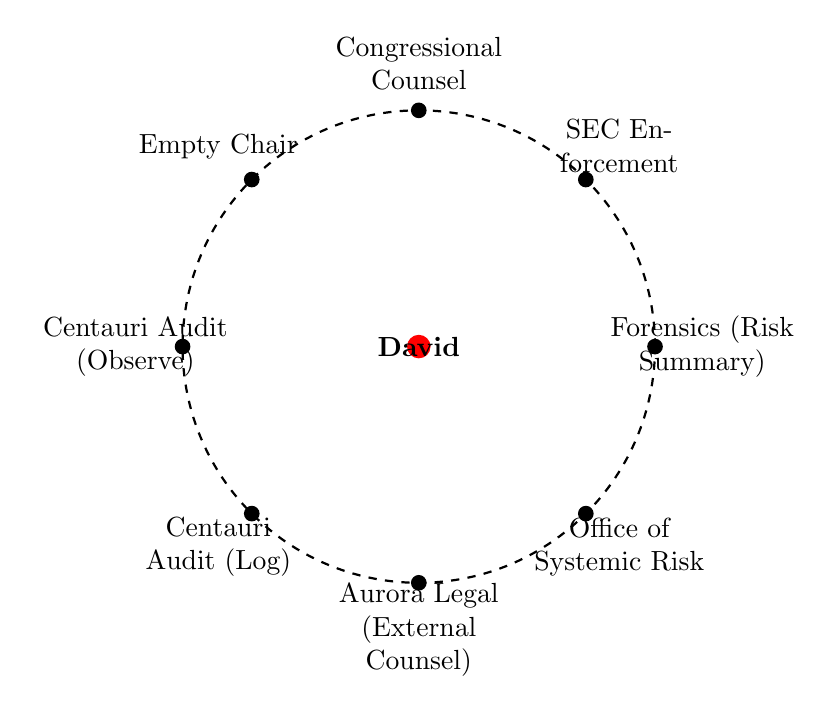
\begin{tikzpicture}
  
  % Draw circular table
  \draw[thick, dashed] (0,0) circle (3cm);
  
  % Define positions
  \foreach \angle/\name in {
      90/{Congressional Counsel},
      45/{SEC Enforcement},
      0/{Forensics (Risk Summary)},
      -45/{Office of Systemic Risk},
      -90/{Aurora Legal (External Counsel)},
      -135/{Centauri Audit (Log)},
      180/{Centauri Audit (Observe)},
      135/{Empty Chair}
  } {
      \node[circle, fill=black, inner sep=2pt] at ({3*cos(\angle)}, {3*sin(\angle)}) {};
      \node[align=center, text width=2.5cm] at ({3.6*cos(\angle)}, {3.6*sin(\angle)}) {\name};
  }
  
  % Center (David)
  \node[circle, fill=red, inner sep=3pt, label=center:{\textbf{David}}] at (0,0) {};
  
  \end{tikzpicture}
  \end{adjustbox}
  \caption{Internal Review Suite -- Seating Diagram}
\end{figure}

\medskip

The room wasn’t loud. It didn’t need to be.

There was no shouting and no drama. It was just methodical and unrelenting questioning. It was the kind 
of questionint designed to wear a man down by inches.

David adjusted his cuff.

He wasn’t in a courtroom.

Not yet.

But the walls were thick. The doors had locks. And the floor felt like it was tilting 
gently underfoot. It was like 
the kind of tilt that says: You’re not walking out of here clean.

\medskip

\begin{TechnicalSidebar}{Due Diligence, Delegation, and the Architecture of Deniability}

  David Morales believed he was protected.  
  Aurora wasn’t the contracting party. The deployment was Centauri’s. The Delaware LLC offered corporate insulation.  
  But legal shields only hold when due diligence is intact.
  
  \medskip
  
  In regulatory doctrine, \textbf{limited liability} and \textbf{role separation} are not get-out-of-jail-free cards —  
  they are privileges that assume \textit{reasonable care within one's domain}.

  \medskip
  
  Morales, as technical validator, was expected to:

  \medskip
  
  \begin{itemize}
    \item Identify and escalate model anomalies,
    \item Document suppressed signals or internal uncertainty,
    \item Ensure executive briefings were technically truthful — not just politically convenient.
  \end{itemize}

  \medskip
  
  He failed in each.  
  He didn’t lie. He didn’t conspire.  
  But he clicked “approve” on a model he knew was incomplete — and that single act converted risk into exposure.
  
  \medskip
  
  \textbf{Michael Hart}, by contrast, had engineered something else entirely:  
  \textbf{plausible deniability by design}.

  \medskip
  
  Centauri owned the deployment.  
  Aurora owned the code — but not the contract.  
  Hart held no formal role in the decision tree. He was the architect, not the executor.
  
  \medskip
  
  He didn’t need to sign anything.  
  He just needed to stage the room, whisper the timelines, and let someone else do the nodding.
  
  \medskip
  
  To a regulator, Morales was the approval trail.  
  To a court, Hart was just an advisor.  
  This was the genius of the structure: \textbf{accountability flowed downhill, but control flowed up.}
  
\end{TechnicalSidebar}

\medskip
